\chapter{General discussion and future directions\label{chap:discussion}}

\begin{remark}{Outline}

In this thesis, we presented three pieces of work that revolve around modeling evolution as a CTMC process in a phylogenetic context. 
First, we demonstrated how we can relax the time-homogeneity assumption in a Bayesian phylogenetic framework leading to the identification of changing sequence and trait evolutionary processes through time.
Next, we introduced a novel simulation architecture that closely matches the model developments in the Bayesian framework we contribute to.
Finally, we complemented the Bayesian phylogeographic inference framework with an easy-to-use visualization software to assist the practitioner in interpreting spatiotemporal reconstructions.
In this concluding chapter, we put several aspects of the presented work into a wider perspective, and we discuss possible extensions in more detail. 

An important part of the work in this thesis is motivated by the need to relax the standard phylogenetic assumptions in search of more biologically plausible models. 
In that respect the work on the time-heterogeneous modeling, presented in Chapter~\ref{chap:epoch}, can be viewed as a first step towards a broader range of models that tackle different types of time-heterogeneity.
We highlight one possible extension of the epoch model, in which time changes in a non-linear fashion.
We then discuss the possibility of inferring both the time and the number of change-points, or transition times, in the epoch model specification via Dirichlet process priors, on which we elaborate in the second section of this summarizing chapter. 

One of the epoch applications focused on the use of codon substitution models to investigate changing selective pressures in HIV evolution within hosts.
Due to their computational burden, the development of codon substitution model extensions in Bayesian phylogenetic inference involving random trees has remained limited.
Motivated by the evolutionary insights that dedicated codon substitution models can provide and by the computational speed-ups we achieved in the epoch inference through fine-grained and coarse-grained parallelization, we are now starting to explore flexible codon model parameterizations in our framework.  
We highlight some of the ongoing work in which we adopt Dirichlet process priors in order to model among-branch and among-site variation in the codon substitution process.

A substantial portion of the work presented in this thesis is devoted to the development of flexible, easy-to-use software.
%GB: perhaps better to specify more clearly what you mean with phylogenetic and population models?
We therefore elaborate on the continued effort to support and extend the $\pi$BUSS simulation software (see Chapter~\ref{chap:pibuss}), with an ever-growing array of phylogenetic and population models.

Highly dimensional estimates that result from Bayesian inference of viral spread in both time and space require dedicated software capable for producing visualizations that are both visually attractive and insightful.
For this purpose, we designed the SPREAD software.
Because the application note on SPREAD we reproduce in Chapter \ref{chap:spread} provides only a brief account of the software, we here take the opportunity to explain the conceptual approach of our spatiotemporal visualizations in more detail, and position them among other approaches.
We also discuss the future directions that we would like to take with the next releases of the SPREAD software, ensuring that it continues to provide the users with an intuitive and user-friendly interface as well as access to a variety of visualization possibilities.

Finally we outline challenges and opportunities that the future might bring in the era of the so-called `genomics plenty', where vast amounts of molecular data can be sequenced increasingly faster and at lower costs, and the high-performance computing strategies that are required to keep up with this data abundance.
\end{remark}

%%%%%%%%%%%%%%%%%%%%%%%%%%%%%%
%---EPOCH MODEL EXTENSIONS---%
%%%%%%%%%%%%%%%%%%%%%%%%%%%%%%
\section{Extending the Epoch model\label{sec:extend_epoch}}

In Chapter~\ref{chap:epoch} we presented a time-heterogeneous substitution model, for which the different types of substitution rates %of evolution
remain constant across all lineages in any given epoch, but vary between those epochs.
We have demonstrated the validity of the method using simulations, and its applicability to empirical HIV and influenza data sets.
We have stressed that by implementing the model as part of Bayesian framework we are able to incorporate uncertainty in the tree reconstruction into our analysis, and thus avoid the need to fix the tree topology or any other evolutionary parameters.

\subsection{Approximating non-linear functions of rate change in time\label{sub:nonlinear}}

For some classes of problems the substitution rates might not vary linearly, at the defined change-points, but rather as some arbitrarily complex function of time. 
Such functions may be difficult, or computationally demanding, to fit exactly and the epoch model may offer an approximate solution to this types of problems.
Let us consider an interval $\left[0,T\right]$ and let the elements of the substitution rate matrix $\mathbf{Q}$ vary independently as an integrable function of time, such that $\mathbf{Q}=\mathbf{Q}(t),\; t\in\left[0,T\right]$. 
The finite-time transition probabilities can be then calculated as: 

\begin{equation}
\ensuremath{\mathbf{P}}(r,T)=exp\left(r\int_{0}^{T}\mathbf{Q}(t)dt\right).\label{eq:rodrigo}
\end{equation}

\noindent
\citet{Rodrigo2008} propose a numerical approximation to $\int_{0}^{T}\mathbf{Q}(t)dt$. 
By taking points $t_{0},t_{1},\ldots t_{n}\in[0,T]$ such that $0=t_{0}<t_{1}<\ldots<t_{n}=T$ and dividing the interval $\left[0,T\right]$ into sub-intervals $\left[t_{i-1},t_{i}\right],\; i=1,\ldots n$ of length $\triangle t_{i}=t_{i}-t_{i-1}$ we have that:   

\begin{equation}
\int_{0}^{T}\mathbf{Q}(t)dt\approx\underset{i=0}{\overset{n}{\sum}}\mathbf{Q}(t_{i}^{*})\cdot\triangle t_{i},\; t_{i}^{*}\in[t_{i-1},t_{i}].\label{eq:approx}
\end{equation}

\noindent
From Equations~(\ref{eq:rodrigo}) and (\ref{eq:approx}), by the definition of the Riemann integral we have that $\mathbf{P}(r,T)=\underset{n\rightarrow\infty}{lim}\underset{i=0}{\overset{n}{\prod}}\text{exp}\left(r\mathbf{Q}(t_{i}^{*})\cdot\triangle t_{i}\right)$, given that rate matrices $\mathbf{Q}(t_{i}^{*})$ commute 
and are closed with respect to the matrix multiplication.
\citet{Sumner2012} formalize the problem of multiplicative closure of the Markov models. 
Given those regularity conditions, we can perform a numerical approximation of any function of rate change by using the epoch time-discretization, and by partitioning the time interval into a fine grid of intervals.
Extending our Bayesian epoch model implementation to accommodate complex rate change functions could be the focus of future work when confronted with a problem that would benefit from such an approach.

\subsection{Evaluating the number and placement of change-points in time}

Both problems presented in Chapter~\ref{chap:epoch}, i.e. HIV within-host evolution before and after progression time and seasonal influenza migration represent hypotheses that condition on a particular number and placement of the transition times.
There might however be a class of problems for which those change points are not known and need to be estimated.
% it remains interesting to investigate possible extensions that estimate the number and position of change points.
A first approach that comes to mind is to introduce an arbitrary number of transitions and estimate their times using the standard MCMC framework.
This straight-forward approach may however not be flexible enough when the number of transition times is small or it may result in
inflated variances when the number is too large. For some problems, e.g. viral diffusion between discretely sampled geographical locations, there is only a single observation per taxon, and this data sparseness might further complicate accurate inference.
Dirichlet Process Priors (DPP) may offer a solution to arrive at efficient estimation of the number and placement of transitions in the epoch model. 
In Subsection \ref{sub:dpp} we further discuss this interesting class of non-parametric prior distributions that we are currently exploring to infer variable selection pressures among lineages using codon substitution models.
%At the time of writing this chapter we are testing these possibilities, yet exactly how accurate the inference of the transition times can be, and how we can quantify the predictive value of those covariates remains an open question for future studies.

\subsection{Introducing covariates in the epoch model\label{sub:glm_epoch}}

In order to test which factors explain the variation in an evolutionary parameter over time, we are currently exploring a \emph{mixed effects} modeling approach. 
Using hierarchical modeling we can introduce random effects for the evolutionary response variable \citep{Edo-Matas2011}.
Assuming effects are additive on the log-scale, we can complete the mixed effects model by incorporating fixed effects to model the impact of covariates on the evolutionary parameters. 

\myedit{svtwenty}{
Specifically we parametrize each epoch specific, possibly multidimensional parameter $\Theta_{i},\; i=1,\ldots,M$ as a log-linear function of $P$ predictors $\mathbf{X}=\left(\mathbf{x_1},\ldots,\mathbf{x_P} \right)$:
}

\begin{align}
log\left(\Theta_{i}\right)=\beta \mathbf{X} \delta+\varepsilon_{i},\; i=1,\ldots,M,
\label{eq:mixed_model}
\end{align}

\noindent
where following the standard terminology in hierarchical modeling, the random effects $\varepsilon_{i}$ quantify different parameter values for each epoch.
$\mathbf{\beta}=\left(\beta_1,\ldots,\beta_P \right)^T$ represent the fixed effects and quantify contribution of a particular predictor to the dependent variable and we assume that:  

\begin{equation}
\beta \sim \text{MVN}(\boldsymbol{\mu},\boldsymbol{\Sigma})
\label{eq:beta_proposal}
\end{equation}

\noindent
The $\left(\delta_1,\ldots,\delta_P \right)$ are binary indicator variables, on which we put independent Bernoulli priors:

\begin{equation}
\delta_{i} \sim \text{B}\left(1,p\right),\;i=1,\ldots,P.
\label{eq:indicator_prior}
\end{equation}

\noindent
The prior specification in Equation~\ref{eq:indicator_prior} allows for Bayesian stochastic search variable selection (BSSVS), which estimates posterior probabilities of inclusion or exclusion of a particular predictor in Equation~\ref{eq:glm} \cite{Lemey2009}.

This represents an important data integration step, for which we have ample experience \citep{Edo-Matas2011,Streicker2012,Vrancken2014} and that will, for example, provide the opportunity to assess the association between within-host HIV evolutionary dynamics and clinical parameters (such as CD4 counts or viral load). 
This will lead to more direct testing of hypotheses that attempt to explain HIV divergence stabilization close to the onset of AIDS (e.g., the cellular exhaustion or immune relaxation hypotheses, \citep{Lemey2007}) by allowing us to test the impact of various predictors in the course of the disease progression.
By using a different parametrization of codon model, such as the GY94 model, parametrized in terms of both the synonymous and non-synonymous rates of substitution, described in Subsection~\ref{sub:dpp} we would be able to disentangle the correlation between synonymous and non-synonymous selection parameters, something that offers an improvement over the approach presented in Chapter~\ref{chap:epoch}.



%%%%%%%%%%%%%%%%%%%%%%%%%%%%%%%%%%%
%---DPP PRIORS FOR CODON MODELS---%
%%%%%%%%%%%%%%%%%%%%%%%%%%%%%%%%%%%
\section{Heterogenous models of codon evolution\label{sub:dpp}}

%\subsection{Introduction}

In Chapter \ref{chap:epoch}, we `epochized' codon substitution models in order to evaluate changing selective pressure in within-host HIV evolution. 
This indicates that flexible modeling of codon evolution may provide important biological insights. 
Their application in a Bayesian phylogenetic context has however been limited due to computational restrictions. 
As also demonstrated by our work, GPU computing now offers the opportunity to push the limits of phylogenetic likelihood computation for high state-space models. 
Our work therefore provides a motivation for codon model developments in the Bayesian framework, and below, we discuss the efforts in this direction that we are currently undertaking.

We are implementing a general form of the Muse \& Gaut (MG94) codon substitution model \citep{Muse1994} that explicitly parameterizes synonymous $\alpha$ and non-synonymous substitution rates $\beta$ by defining the instantaneous rate of replacing codon $i$ with codon $j$ ($i \neq j$) as follows:

\begin{displaymath}
q_{ij}^{MG} = \begin{cases} \theta_{mn,s}\alpha_{s}^{b}\pi_{n}^{p}, & i \to j \text{ is a one-nucleotide synonymous substitution} \\ & \text{from nucleotide $m$ to nucleotide $n$ in codon position $p$,} \\ \theta_{mn,s}\beta_{s}^{b}\pi_{n}^{p}, & i \to j \text{ is a one-nucleotide non-synonymous substitution} \\ & \text{from nucleotide $m$ to nucleotide $n$ in codon position $p$,} \\ 0, & \text{otherwise.} \end{cases}
\end{displaymath}

$\pi_{n}^{p}$ denotes the frequency of nucleotide $n$ in codon position $p = 1,2,3$. 
As denoted by the sub/superscript, synonymous and non-synonymous substitution rates $\alpha_{s}^{b}$ and  $\beta_{s}^{b}$ may depend on both the alignment site ($s$) and the branch of the tree ($b$). 
Parameter $\theta_{mn,s}$ corrects for the nucleotide substitution bias. 
Setting all $\theta_{mn,s}$ equal to 1 and assuming no rate variation among sites or branches reduces the model to the original Muse \& Gaut codon model.% \citep{Muse1994}.

Whereas a homogeneous MG94 model is relatively straightforward to estimate, it most likely constitutes an oversimplification, as there is no biological reason to assume that the selective pressures are the same for any two branches or any two sites.
To incorporate among-lineage variation in both $\alpha$ and $\beta$, the most flexible, but likely over-parameterized, approach would be to consider a separate MG94 for each branch in the phylogeny.
This would however be computationally impractical to fit to large size data sets, because it requires an eigen-decomposition of the infinitesimal generator for each branch.
Specifying different substitution models for different time intervals or epochs throughout the evolutionary history, which we demonstrated using a Goldman and Yang codon substitution model \citep{Goldman1994} in BEAST, provides one way of introducing heterogeneity through time, while keeping the computation time manageable (Chapter~\ref{chap:epoch}). 

%FB: typical notation  DP(G_0,\gamma)
Although the epoch model is useful as a specific case of allowing for variation in $\alpha$ and $\beta$ throughout evolutionary history, more general approaches would be desirable.
We are currently developing novel Bayesian non-parametric priors specifically tailored for evolutionary problems to hold the middle ground between the homogeneous MG94 model and estimating a separate MG94 model for each branch/site.
Bayesian non-parametric priors are often employed in problems where one wishes to cluster unknown parameters into distinct classes without making strong distributional assumptions.
The most common is the \emph{Dirichlet process} (DP) prior. 
In phylogenetics, this model has been developed for modeling among-site variation in the rates of non-synonymous substitutions \citep{Huelsenbeck2006} and to model lineage-specific substitution rates by assigning branches to rate categories \citep{Heath2012}.
A Dirichlet process DP$(F, \alpha)$, where $F$ (the base distribution) is a single parametric distribution and $\alpha$ (the concentration parameter) is a positive real number, returns a random distribution that is an infinite mixture of $F$ with different base parameters, e.g.~means and variances.
The partitioning of branches into specific realized values, called categories, is controlled by the concentration parameter $\alpha$, where small values of $\alpha$ lead to fewer categories and greater homogeneity of the substitution process, whereas large values indicate increased branch- or site-specific substitution processes.
Whereas often a single (branch- or site-specific) parameter is drawn from the base distribution $F$, our approach for the MG94 model requires two of such parameters to be drawn, for which we propose to first adapt the suggested DP prior.
A limitation of the DP is that there is no natural ordering for its realizations; any two draws share the same correlation.  
On an evolutionary history, this assumption is unrealistic; Thorne et al.~\citep{Thorne1998}, Seo et al.~\citep{SKT04} and Aris-Brosou and Yang \citep{Aris-Brosou2002} have long argued for phylogenetic auto-correlation among branch-specific rates.
We propose to achieve both auto-correlation and non-parametric flexibility by extending DPs to have first-order dependence along the evolutionary history.  
To accomplish this, recent work in Bayesian inference with DPs and their generalization, \emph{Polya urns}, \citep{Guha2010} shows that \emph{infinite hidden Markov models} \citep{Beal2002} in the computer science literature are now as convenient to fit as DPs and will allow for dependence across neighboring branches while retaining their non-parametric behavior.

\begin{remark}{Infinite Hidden Markov models\label{ref:infinite_hidden_markov}}
A Hidden Markov model (HMM) $\left\{ X\left(t\right):\; t=1,2,\ldots\right\}$ defines a probability distribution over sequences of observations $\mathbf{X}=\left\{ X(1), \ldots,X(t) \right\}$ by invoking another sequence of unobserved (\emph{hidden}) discrete state variables $\left\{ C\left(t\right):\; t=1,2,\ldots\right\}$.
 
% Let us denote the past states of these processes  from time $1$ to time $t$ by 
The model is defined by three parts: first the \emph{transition matrix} of the hidden process, which satisfies the Markov property, i.e.:

\begin{align}
% \mathbf{P}=\left\{ p_{ij}\right\} ,\text{where }p_{ij}=&P\left\{ C\left(t\right)|C\left(t-1\right),\ldots,C\left(1\right)\right\} \nonumber \\ 
% =&P\left\{ C\left(t\right)|C\left(t-1\right)\right\} , 
\mathbf{P}=\left\{ p_{ij}\right\} ,\text{where }p_{ij}=& P\left\{ C\left(t\right)=j|C\left(t-1\right)=i,C\left(t-2\right),\ldots \right\} \nonumber \\ 
=& P\left\{ C\left(t\right)=j|C\left(t-1\right)=i\right\} 
\label{eq:hmm_trans}
\end{align}

\noindent
secondly the \emph{emitting matrix} of the `state-dependent process', which depends only on the current state of the hidden process and not on the previous states, i.e.:

\begin{align}
% \mathbf{X}=\left\{ x_{ij}\right\} ,\text{where }x_{ij}=& P\left\{ X\left(t\right)|C\left(t\right),X\left(t-1\right),\ldots,X\left(1\right)\right\} \nonumber \\
% =&P\left\{ X\left(t\right)|C\left(t\right)\right\} ,
\mathbf{X}=\left\{ x_{jk}\right\} ,\text{where }x_{jk}=& P\left\{ X\left(t\right)=k|C\left(t\right)=j,X\left(t\right),X\left(t-1\right),\ldots \right\} \nonumber \\
=&P\left\{ X\left(t\right)=k|C\left(t\right)=j\right\} ,
\label{eq:hmm_emit}
\end{align}

\noindent
and lastly the vector of starting probabilities of being in some state $i$ at the beginning, i.e.:

\begin{align}
\Pi=\left\{ \pi_{i}\right\} ,\text{where }\pi_{i}=P\left\{ C\left(t=1\right)=i\right\} 
\label{eq:hmm_start}
\end{align}

\noindent
If the Markov chain $\left\{ C\left(t\right) \right\}$ has $m$ states we call $\left\{ X\left(t\right) \right\}$ an $m$-state HMM and $\lambda=\left(\mathbf{P},\mathbf{X},\Pi\right)$ is typically used as a compact notation for an HMM.
Extending the \emph{hidden} $\left\{ C\left(t\right) \right\}$ process to a countably infinite number of hidden states for leads to the infinite HMM's.
\end{remark}

We are pursuing such among-branch approaches and will adopt similar non-parametrics to model among-site variability in $\alpha$ and $\beta$. 
These developments will yield powerful tools to uncover variable selection pressure in coding sequences for many different pathogens, as well as other organisms.
Moreover, they will be essential to accurately estimate time-scales for viral evolutionary histories where standard evolutionary models lead to divergence time underestimation \citep{Wertheim2011}. 
Such a bias has been attributed to the action of strong purifying selection over long evolutionary time scales, and selection-informed models have been shown to improve branch length estimation \citep{Wertheim2011}, but their implementation in phylogenetic dating software is still lacking.




%Codon substitution models were independently proposed by \cite{Muse1994} and \cite{Goldman1994} in the same issue of Molecular Biology and Evolution (MBE).
%In these models, a non-stop codon triplet $n_{1}n_{2}n_{3}$ is considered as the smallest unit of evolution.
%According to the universal genetic code, there are $4^3$ possible triplets minus three stop codons, resulting in a state space size of $61$ codons.
%The standard assumption of independence is used, i.e. the substitutions at these three codon positions occur independently, and only a single change per triplet can occur at a given time. 
%%GB: explain in more detail, i.e. more than 1 change is possible in subsequent infinitesimal time intervals
%%GB: are there no codon models that allow for multiple substitution per time unit (I thought I recently read something like that ... will look it up and send e-mail)
%Proteins are coded by a set of 20 amino acids, with each amino acid being coded by a codon triplet. 
%Because there are 61 non-stop codons to encode for 20 amino acids, some amino acids will inevitably be coded by more than 1 codon.
%A substitution that does not change the encoding amino-acid is called a synonymous substitution, while a non-synonymous substitution refers to a substitution that does result in an amino acid substitution.
%
%Selective pressure is the main force behind molecular evolution.
%Understanding and inferring the selective pressure is one of the central goals of molecular virology, see for example \citet{Bielejec2014a}.
%That is why most of the codon substitution models are parameterized in terms of the rate of non-synonymous (denoted by convention $\beta$) and synonymous ($\alpha$ by convention) substitutions.
%Their ratio $\omega=\beta / \alpha$ is a standard measure of the selective pressure \citep{ThePhylogeneticHandbook}, which is sometimes also denoted $\omega = dN/dS$.
%Prevalence of synonymous substitutions over non-synonymous ones leads to a \emph{purifying (negative)} selection, and corresponds to the ratio $\omega <1$.
%If non-synonymous substitutions accumulate at a faster rate than the synonymous substitutions this is coined \emph{positive selection}, improving the fitness of the particular organism.
%$\omega\approx 1$ signifies neutral evolution.
%
%There are several advantages in using codon models over nucleotide-based substitution models.
%Not all DNA positions evolve at the same rate, with non-synonymous substitutions occurring more frequently then synonymous substitutions.
%Although this problem can be mitigated to some extent by using codon-positioned nucleotide substitution models, the fast evolving positions and the state space limited to 4 character alphabet still can lead to biased estimates over long evolutionary distances, as portrayed in the previous Chapter~\ref{chap:pibuss}.
%
%% GY style models
%The model proposed by \cite{Goldman1994} is characterized by a substitution rate matrix with following entries:
%
%\begin{equation}
%\left\{ \mathbf{Q}\right\} _{ij}=\begin{cases}
%\pi_{j} & \substack{ \text{ \ensuremath{i\rightarrow j} is a synonymous transversion from } \\ \text{codon \ensuremath{i} to \ensuremath{j} } } \\  
%\kappa\cdot\pi_{j} & \substack{ \text{ synonymous transition } } \\
%\omega\cdot\pi_{j} & \substack{ \text{ non-synonymous transversion } } \\
%\omega\cdot\kappa\cdot\pi_{j} & \substack{ \text{ non-synonymous transversion } } \\
%0 & \substack{ \text{ otherwise} }
%\end{cases},
%\label{eq:gy94}
%\end{equation}
%% % {\footnotesize
%% \begin{equation}
%% q_{ij}^{GY94}=\begin{cases}
%% \pi_{j} & \text{if \ensuremath{i\rightarrow j} is a synonymous transversion}\\
%% \kappa\cdot\pi_{j} & \text{if \ensuremath{i\rightarrow j} is a synonymous transition}\\
%% \omega\cdot\pi_{j} & \text{if \ensuremath{i\rightarrow j} is a non-synonymous transversion}\\
%% \omega\cdot\kappa\cdot\pi_{j} & \text{if \ensuremath{i\rightarrow j} is a non-synonymous transversion}\\
%% 0 & \text{otherwise}
%% \end{cases},
%% \label{eq:gy94}
%% \end{equation}
%% % } % END: size
%
%\noindent
%where the parameter $\kappa$ denotes the transition/transversion ratio, parameter $\omega$ denotes the non-synonymous/synonymous
%rate ratio and $\pi_j$ denotes the equilibrium frequency of codon triplet $j$.
%The parameters $\kappa$ and $\pi_j$ can be thought of as controlling the CTMC process at the DNA level, while the $\omega$ parameter characterizes the selection on non-synonymous substitutions.
%For the GY94 model the synonymous evolutionary rate is fixed to be 1, i.e. $\omega=\beta$.
%
%Different flavours of the GY94 model differ in the composition of the equilibrium codon frequency parameter $\pi_{j}$.
%One approach is to model the codon frequencies as each having the same long-time frequency of appearing. 
%Such model is referred to as the GY94-Fequal.
%
%In the GY94-F$1\times4$ model codon frequencies are calculated from the four nucleotide frequencies, with frequencies being pulled from all three codon positions, i.e. $\pi_{n_{1}}=\pi_{n_{2}}=\pi_{n_{3}}$ for all four nucleotides,.
%This model leads to 3 free parameters that need to be estimated from the data. 
%%GB: they're often not estimated during the MCMC run, but empirical values are used.
%%GB: how are these 'nucleotide frequencies' then used to calculate the 'codon frequencies' ?
%If the frequencies are parameterized according to three sets of nucleotide frequencies for the three codon positions, resulting in nine free parameters, the model is called the GY94-F$3\times4$.
%Finally in the GY94-F61 model every codon triplet has it's own frequency parameter, with all parameters summing to one, resulting in 60 free parameters that need to be estimated.
%
%The GY94-F61 model has been suggested as important in letting the model explain the data without constricting assumptions.
%\citet{Rodrigue2008} however argue that the model has no interpretation on the nucleotide level as well as confounds other effects inducing uneven codon stationary probabilities.
%The authors criticize the GY94-F$3\times4$ setup as superficial, pointing that the periodic pattern along the nucleotide sequence positions represents the coding structure of the sequence but not the processes that shape the evolution.
%
%% MG style models
%The Markov generator matrix for MG94 style models \citep{Muse1994} is given by:
%
%\begin{equation}
%\left\{ \mathbf{Q}\right\} _{ij}=\begin{cases}
%\alpha\cdot\kappa\cdot\pi_{n}^{p} & \substack{ \text{ \ensuremath{i\rightarrow j} is a synonymous transition from } \\ \text{nucleotide \ensuremath{m} to \ensuremath{n} at codon position \ensuremath{p} } } \\
%\alpha\cdot\pi_{n}^{p} & \substack{ \text{ synonymous transversion from } \\ \text{\ensuremath{m} to \ensuremath{n} at position \ensuremath{p} } } \\
%\beta\cdot\kappa\cdot\pi_{n}^{p} & \substack{ \text{ non-synonymous transition from } \\ \text{\ensuremath{m} to \ensuremath{n} at position \ensuremath{p} } } \\
%\beta\cdot\pi_{n}^{p} & \substack{ \text{ non-synonymous transversion from } \\ \text{\ensuremath{m} to \ensuremath{n} at position \ensuremath{p} } } \\
%0 & \substack{ \text{ otherwise}}
%\end{cases}.
%\label{eq:mg94}
%\end{equation}
%
%There are two main differences to be noted with respect to the GY94 style codon models.
%First, the model is parameterized in terms of both the non-synonymous ($\beta$) and synonymous ($\alpha$) rates, meaning that a change in the ratio may be due to alteration of the rate of non-synonymous or synonymous substitutions, or both.
%Second, the model estimates the frequencies of the target nucleotide $\pi_{n}^{p}$ rather than of the target codon triplet $\pi_{j}$, as in the GY94 model.
%As before the MG94 model can be used with frequencies specified as a single (MG94-F$1\times4$) or three (MG94-F$3\times4$) vectors with 4 dimensions.
%For the remainder of this chapter we will focus our estimation on the MG94 parameterization, mostly because the parameterization in terms of both the synonymous and non-synonymous substitution rates offers interesting opportunities for disentangling the patterns of correlation between the two.
%
%% first talk about across site variation
%%GB: when you say constant, do you mean homogeneous?
%Molecular phylogenetic analyses using codon models are typically restricted to fitting a single model, with constant parameterization across data, i.e. sites of the alignment.
%However there is no biological reason to assume that all the sites are under the same selection regime.
%\cite{NY98} point towards the fact that for most real world data sets, of which we know that they evolved under positive selection pressure only a handful of sites actually contributed towards the non-synonymous to synonymous rates ratio >1.
%%GB: replace constant with homogeneous?
%Therefore, applying constant model to the data, without accounting for across-data heterogeneity, biases the estimates of $dN/dS$ ratio towards lower values.
%In some cases this might lead to a failure in detecting positive selection even if it's actually present in the data.  
%In that respect \cite{NY98} propose two models in the GY94 context, with a fixed number of categories to which a particular site can belong.
%Their \emph{neutral model} assumes a category for sites where the non-synonymous mutations are neutral ($\omega_1=1$) and a category for sites which are conserved ($\omega_2=0$).
%Their \emph{positive selection model} adds an extra category of positively selected sites ($\omega_3>1$).
%\cite{Goode2008} employ this setup and further extend it by allowing for a change in $\omega$ parameter value at some specified time between the most-recent common ancestor and the most recent sampling time.
%
%These models, although undeniably a step in the right direction, still make strong assumptions, among which partitioning sites into a fixed number of rate classes and estimating the rate for each class separately is probably the most restrictive one.
%Ideally, the model should let the data decide how many rate classes there are, and what the site-specific values are.
%
%A first modelling approach that comes to mind is to fit a different rate to each site in the alignment \citep{Nielsen1997}.
%Although this approach might seem naive at first, it bears a valuable property in that no explicit assumption in the distribution of rates across sites is being made.
%However other negative factors still persist, precluding such a class of methods from being generally applicable.
%The main problem is that, particularly for long sequences, many parameters need to be estimated, increasing the computational costs.
%In case of shorter sequences such a method may overfit the data, leading to a significant loss of statistical power and biased estimates.
%Another approach treats site-specific rates as independent draws from some common distribution, e.g. a gamma distribution \citep{Yang1993} or inverse Gaussian probability distribution \citep{Waddell1997}, sometimes with a proportion of sites allowed to remain invariable \citep{Gu1995}.
%This approach allows to model the rate variation with relatively few parameters, as well as provides pooled estimates of the distribution parameters, which can in turn be compared across different data-sets.  
%In many scenarios though a single parametric distribution proves too naive of an approach to capture complex patterns of rate evolution \citep{Pond2005a}.
%\cite{Yang2000} proposed to model among-site substitution rate variation in codon models by employing a mixture of different distributions.
%Although mathematically possible, this proved computationally too expensive to fit mixtures of continuous distributions for the parameters of interest and the authors resort to fitting discrete approximations.
%Although these constraints are being actively stretched \citep{Suchard2009,Ayres2012}, averaging over a large array of distributions remains computationally intensive. 
%\citet{Pond2005a} propose a simple, yet flexible model of rate variation with an integrative method to reliably estimate the fluctuating parameters.
%This method proceeds by partitioning the rate distribution into a countable number of intervals, with each interval represented by some statistic.
%%GB: explain this beta model thingy
%Then a beta model is used to decide what intervals the underlying rate distribution is partitioned into and calculate corresponding rate class values.
%This is perhaps the most flexible approach for evaluating site-specific rate variation to date, that provides a good fit to data with only a few extra parameters.
%
%\cite{Heath2012} introduces a model which relaxes the assumption of a strict molecular clock in a way that is alternative to the Random Local Clock models (\cite{Drummond2010}, see Subsection~\ref{sub:clocks}), which proceed by clustering branches on a tree which share the same rate.
%In the approach proposed by \cite{Heath2012} both the number of the rate classes, as well as their placement are modeled using a Dirichlet process prior (DPP, \cite{Ferguson1973}). % which treats them as random variables.
%Here we propose an approach which is similar in spirit to \cite{Heath2012}, although our interest lies not in modelling overall branch rates, but in modelling across-lineage heterogeneity of the parameters of codon substitution models, such as the synonymous and non-synonymous substitution rates.
%
%Both the number and the clustering of the lineage-specific parameters are treated as random, and are controlled by a Dirichlet Process Prior.
%A DPP is a "distribution over distributions" and induces clusterings with a varying number of components that can grow or shrink depending on the data and a concentration parameter.
%It is thus often used as a prior over possible clusterings where the exact number and population of distinct clusters is not known beforehand.
%We require no structure to be enforced on the clustering of the branches, and allow the data to drive the model in a descriptive fashion. 
%Our only requirement is the prior specification of the concentration parameter of DPP, controlling whether a model prefers less clusters with many occupants or more less densely populated ones. 
%By implementing our model as part of BEAST's Bayesian inference framework we allow for a hyperprior to be put on this parameter to average over all of its possible values. 
%This approach avoids overparameterisation and computational overhead by achieving data-driven balance between simplicity and complexity of the model.
%We use Markov chain Monte Carlo (MCMC) techniques, in which a chain with a memoryless property is constructed to draw samples from the posterior.
%Although we focus our efforts on estimating the patterns of variation in codon substitution models our implementation is generally applicable to any parameters that exhibit across-data or across-time heterogeneity .
%Below we describe the main aspects of the model.
%
%\subsection{Methods}
%
%We use a Dirichlet process prior (DPP) to model branch-specific codon parameters.
%In real-world applications not every branch in the tree would display the same type of evolutonary behaviour, therefore it would be natural to expect some degree of clustering between them.
%Suppose one is interested in a branch-specific parameter $\theta_{i}, i=1,\ldots,N$, where $N=2n-1$ is the number of branches in a tree with $n$ taxa. 
%This parameter might be multi-dimensional, yet for simplicity our notation will be limited to the univariate case.
%We expect \emph{a priori} that $K\ll N$, where $K$ denotes the number of unique clusters of branches.
%All of the branch-specific parameters have the same distribution $B$:
%
%\begin{equation}
%\forall i=1,\ldots,N: \theta_{i}\sim B(\mu_{z_{i}}),
%\label{eq:dpp1}
%\end{equation}
%
%\noindent
%where we will use $\mathbf{z}$ to denote the vector of branch category assignments.
%Each branch receives a category $z_{i},\; i\in\left\{ 1,\ldots K\right\}$, where $K\in\left\{ 1,\ldots,N\right\}$ denotes the a number of branch categories.
%As an example let us consider a topology $\mathbf{F}$ with $N=3$ branches and a fixed number of categories $K=2$.
%One possible realization of the vector of assignments would then be:
%
%$$\mathbf{z}=\left(z(1)=1,\; z(2)=1,\; z(3)=2\right),$$ 
%
%\noindent
%meaning that branches one and two belong to the same category 1, and that the third branch belongs to the category 2.
%Let us denote the uniquely realized branch-specific parameter values by $\hat{\theta_{j}}, j=1,\ldots,K$.
%%GB: what do you mean when you say 'mechanistic' ? Do you mean 'deterministic' ?
%A mechanistic function $f$ keeps track of the mapping between the branches and unique realizations $\hat{\theta_{j}}$:
%
%\begin{equation}
%\mu_{z_{1}},\ldots,\mu_{z_{N}}=f\left(\hat{\theta}_{1},\ldots,\hat{\theta}_{K},z_{1},\ldots z_{N}\right).
%\label{eq:dpp2}
%\end{equation}
%
%\noindent
%The idea behind using DP priors is to set up a kernel distribution with probability distribution function $P_{0}$ from which unique branch-specific candidate values $\hat{\theta_{j}}$ are drawn:
%
%\begin{equation}
%\forall i=1,\ldots,N\;\hat{\theta_{j}}\sim P_{0}\left(\mu\right).
%\label{eq:dpp3}
%\end{equation}
%
%\noindent
%Clustering indicators for each branch are sampled according to a Dirichlet process with intensity $\gamma$:
%
%\begin{equation}
%z_{1},\ldots,z_{N}\sim DP(\gamma).
%\label{eq:dpp4}
%\end{equation}
%
%\noindent
%By defining hyper-priors for the parameters of the kernel distribution and a concentration parameter of the DP, or alternatively fixing them to specific values, we complete the specification of the DPP:
%
%\begin{equation}
%\begin{array}{c}
%\mu\sim P_{1}(\ldots)\\
%\gamma\sim P_{2}(\ldots)
%\end{array}.
%\label{eq:dpp5}
%\end{equation}
%
%% One of them is to consider the branch-specific values as coming from a mixture of distributions
%There are several possible implementations of the Dirichlet process for drawing the cluster indicators as defined in Equation \ref{eq:dpp4}. 
%One of them is the so-called "stick-breaking" construction \citep{Sethuraman94}.
%The draws from a DP are composed of a weighted sum of point masses $P$, summing up to 1 and giving rise to a discrete distribution.
%The algorithm to generate a single draw from DP is given in Listing \ref{alg:stickBreaking}.
%
%\begin{algorithm}[H]
%\begin{center}
%\begin{algorithmic}[1]
%% \footnotesize{
%%
%\State $remainingLength \gets 1.0$;
%%
%\For{$\left( \text{int } j=0; \; j<K; \; j++\right)$}
%%
%\State $r\sim Beta\left(1,\gamma\right)$;
%%
%\State $P\left[j\right]=r \cdot remainingLength$;
%%
%\State $remainingLength=\left(1-r\right) \cdot remainingLength$;
%%
%\EndFor \\
%%
% \textbf{return} $P$;
%% }
%\end{algorithmic}
%\end{center}
%\caption{ 
%{ \footnotesize 
%{\bf Constructing the Dirichlet process by stick breaking.} 
%}% END: footnotesize
%}
%\label{alg:stickBreaking}
%\end{algorithm}
%
%Colloquially we can describe it as follows: we start with a stick of length 1 and break it randomly at point $r_{1}$ chosen by drawing one value from $\text{Beta}(1, \gamma)$ and assign $p_{1}$ to the length of the part of the stick that we just broke off.
%We then recursively break other portions of the stick to obtain $p_{2}, p_{3}, \ldots$ and so forth, each time setting:
%
%\begin{equation}
%p_{i}=r_{i}\cdot\underset{j}{\overset{i-1}{\prod}}\left(1-r_{j}\right).
%\label{eq:sticks}
%\end{equation}
%
%\noindent
%Parameter $\gamma$ controls the clustering behaviour of the process.
%Smaller values will lead to fewer, yet more populated categories; larger values will result in more categories being occupied by less branches.
%
%Under our DPP model both the number of categories $K$ and category assignments $z_{i}$ are random variables, controlled by a DPP with a concentration parameter $\gamma$ and a base distribution given by $P_{0}$.
%The complete likelihood of the model can be written down as:
%
%\begin{equation}
%L(\mathbf{z},K|\gamma,N,\hat{\theta_{1}},\ldots,\hat{\theta_{K}})=\gamma^{K}\cdot\frac{\underset{j=1}{\overset{K}{\prod}}\left(\eta_{j}-1\right)!}{\underset{i=1}{\overset{N}{\prod}}\left(\gamma+i-1\right)}\cdot\underset{j=1}{\overset{K}{\prod}}P_{0}\left(\hat{\theta_{j}}\right)^{\eta_{j}},
%\label{eq:dppLike} 
%\end{equation} 
%
%\noindent 
%where $\eta_{k}$ denotes the number of sites assigned to category $k$.
%%GB: do you want to talk about the increased computational demands of codon models? and how this can be alleviated by using BEAGLE on GPUs?
%%GB: do you w  ant to show a figure that explains the redundancy of the genetic code?
%
%\subsection{Summary}
%% TODO: call it `Summary & Preliminary Results', show some numericla results + plots from tests on the Galaxy data
%
%This model is currently being  implemented in the BEAST software package.
%This pending implementation is currently being tested against an implementation in the JAGS software \citep{Plummer2003}, and we are using a numerical example to compare the results.


%%%%%%%%%%%%%%
%---SPREAD---%
%%%%%%%%%%%%%%
\section{Future prospects for visualizing viral diffusion\label{sec:spread_exten}}

% Genetic and phenotypic data become useful only when we apply methods deriving insights from it, and these methods encompass statistical inference as well as visualization of its results. Visualizing estimates provides an efficient way to communicate results to the scientific community and beyond. Bayesian evolutionary inference, however, generates \textbf{high-dimensional} estimates, e.g. ancestral reconstructions of (multiple) traits on a posterior distribution of trees. When multidimensionality complicates the visualization task, dynamic, interactive visualizations may offer an attractive solution. In our case, the time scale of the evolutionary histories represents a natural dimension to explore for dynamic interactions. Interactivity can also encourage engagement and may lead to a better understanding and even appreciation of the statistical inference procedure itself. 

\paragraph{}
In Section~\ref{sub:clocks} we discussed how past evolutionary events can be estimated in calendar time units by using molecular clock models and historical node calibrations or dated tip calibrations.
A natural representation of the spatiotemporal reconstructions is to animate a `geophylogeny' as it unfolds through time and space.
The visualization of spatiotemporal history, with the possibility to dynamically examine how the diffusion process unfolds, has been the main motivation for the development of SPREAD \citep{Bielejec2011}, presented in Chapter~\ref{chap:spread}.
SPREAD allows for visualizing animated geophylogenies in an automated manner, by producing output in time-annotated Keyhole Markup Language (KML), an ISO standard geographic markup language maintained by the Open Geospatial Consortium that can be read and written by most spatial software. 
KML encoding allows for manipulating virtually all aspects of the mapping: colour and line thickness, height and placement, the type of projection, labeling, etc.
The SPREAD GUI provides the user with control over fine-tuning these parameters and the output can be used in virtual globe software like Google Earth (\url{http://www.google.com/earth/}) or high-end GIS software like ArcGIS or Cartographica.
Here, we take the opportunity to position our visualization approach among others and discuss further directions of SPREAD in more details.

\subsection{Past and current efforts in visualising phylogeography\label{sub:visual}}

Geophylogenies, or more generally geo-trees are spatially referenced phylogenies, for which taxa exist in a real space and can be displayed as cartographic elements within a map \citep{Kidd2010}.   
Possibly the first 
mapping of a phylogeny in a geographical context 
%diagram like that, depicting evolutionary tree over geographical map
is the famous \textit{Hypothetical Sketch of the Monophyletic Origin and the Extension of the 12 Races of Man from Lemuria over the Earth} shown in \cite{Haeckel1876} (see Figure~\ref{fig:lemuria}).
Ernst Haeckel, a XIX century naturalist entertained the idea that the absence of missing fossil links in human evolution at his time could be explained by existence of \textit{Lemuria}, a sunken island in the Indian Ocean.  
% Although the hypothesis obviously did not hold, the phylogenetic visualization has received considerable attention.
%The phylogenetic visualisation has surpassed the, entirely discredited, work itself.
Although the hypothesis obviously did not hold, the phylogenetic visualization has received considerable attention and surpassed the discredited work.

\begin{figure}[h!]
\centering
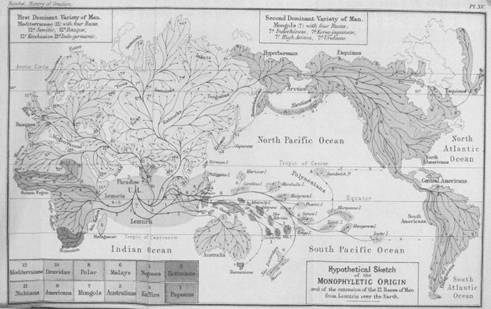
\includegraphics[scale=0.25]{lemuria}
\caption{
{ \footnotesize 
{\bf Hypothetical Sketch of the Monophyletic Origin and the Extension of the 12 Races of Man from Lemuria over the Earth. E. Haeckel, 1876.} 
} % END: footnotesize
}
\label{fig:lemuria}
\end{figure}


% other tools
The joint study of spatial dispersal processes along with the patterns of genomic ancestry has been formalized into the field of phylogeography.
Summarizing the estimates in a clear and concise way is just as important of a step as the statistical analysis itself \citep{Hadley2010}.
This is especially true for complex patterns of biogeographic processes, where visualization is key to interpret and understand them. 
Recently great research effort has been undertaken to visualize the phylogenetic relationships between organisms in relation to their geographic distribution. 

\paragraph{}
In order to visualize the outcome of spatial dispersal and evolutionary history, geographic distributions can be displayed as an annotation on the tree, with tip branches labelled according to the names of the locations from which the samples were obtained.
This can be carried out using advanced tree visualization tools such as FigTree (\url{http://tree.bio.ed.ac.uk/software/figtree/}).
More complex annotations can be displayed in iTOL \citep{itol}, which is capable of displaying charts on the internal or external branches, displaying prevalence of any kind of data, including discrete geographic locations with a scale to reflect its size.
This approach is most appropriate when the geographic complexity is low, as it simplifies the spatial context to text or symbolic representation, therefore prioritizing the ancestral relationship over the spatial process.

\paragraph{}
A more geographically explicit visualization combines cartographic maps with images of trees, such as the so-called `tangle-maps'.
The GenGis software, developed by \cite{Parks2009} supports these types of visualizations (Figure~\ref{fig:tanglemaps}).
%Tangle-maps are visualizations that combine cartographic maps with images of trees.
Although tangle-maps visually link the tree and the map through the use of graphic lines, the tree is merely overlaid on the map and provides little insight into dispersal history.

\begin{figure}[h!]
\centering
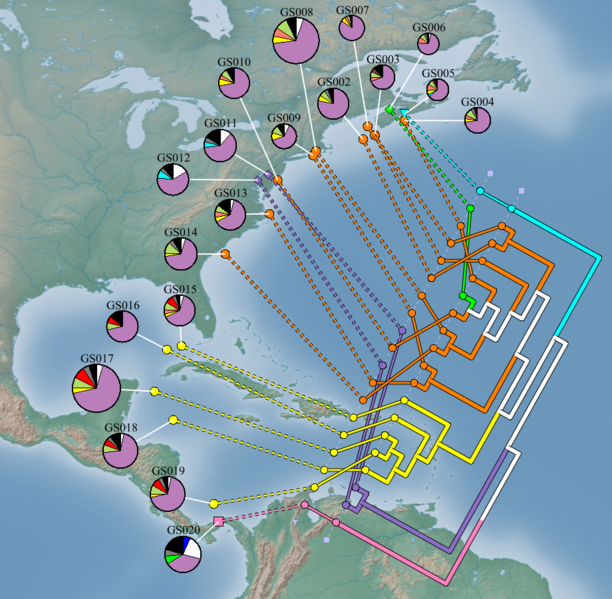
\includegraphics[scale=0.3]{tanglemaps}
\caption{
{ \footnotesize 
{\bf Tangle-map of the biodiversity of 19 marine metagenomes.} 
The figure is plotted using GenGis (\url{http://kiwi.cs.dal.ca/GenGIS/Main_Page}).
} % END: footnotesize
}
\label{fig:tanglemaps}
\end{figure}

% how we do it
\paragraph{}
Through ancestral state reconstruction (see Subsection~\ref{sub:phylogeo}), model-based approaches can provide location estimates at ancestral nodes in the phylogeny as well as their uncertainty, which is crucial for hypothesis testing.
%to phylogenetic reconstruction, such as ancestral state reconstruction (see Subsection~\ref{sub:phylogeo}) provide estimates for phylogeographic relationships, but also the uncertainty in those estimates, which is crucial for hypothesis testing.
Appropriately accommodating statistical uncertainty into phylogeographic visualizations is however a major challenge.
Ancestral location reconstructions allow mapping the entire tree structure, both internal and external nodes, in a geographic context.
In BEAST, location data can be modeled either as finite and countable (discrete) states or bivariate (longitude and latitude) realizations in continuous space.
This choice is mainly dependent on the sampling scheme of the data and the nature of the dispersal process.
Different representations of uncertainty need to be applied in these approaches.
When bivariate coordinates are inferred for the internal nodes using a Brownian motion model, the geographic uncertainty is expressed as confidence envelopes or credible contours for each internal node.
This is illustrated by Figure~\ref{fig:cont}, where a 3D-geophylogeny with credible contours for particular points in time is projected on the surface in Google Earth.
We can only project a single tree from the posterior (e.g. using the mean bivariate location estimates for every node), but the uncertainty can be obtained by slicing each tree in the posterior at a particular point in time and imputing the locations for each branch that is sliced (Figure~\ref{fig:cont} illustrates two time slices).
All these time-specific location estimates can be used to build a credible contour through kernel density estimation.
SPREAD supports such 2D projections based on estimates resulting from a BEAST analysis.

\begin{figure}[h!]
\centering
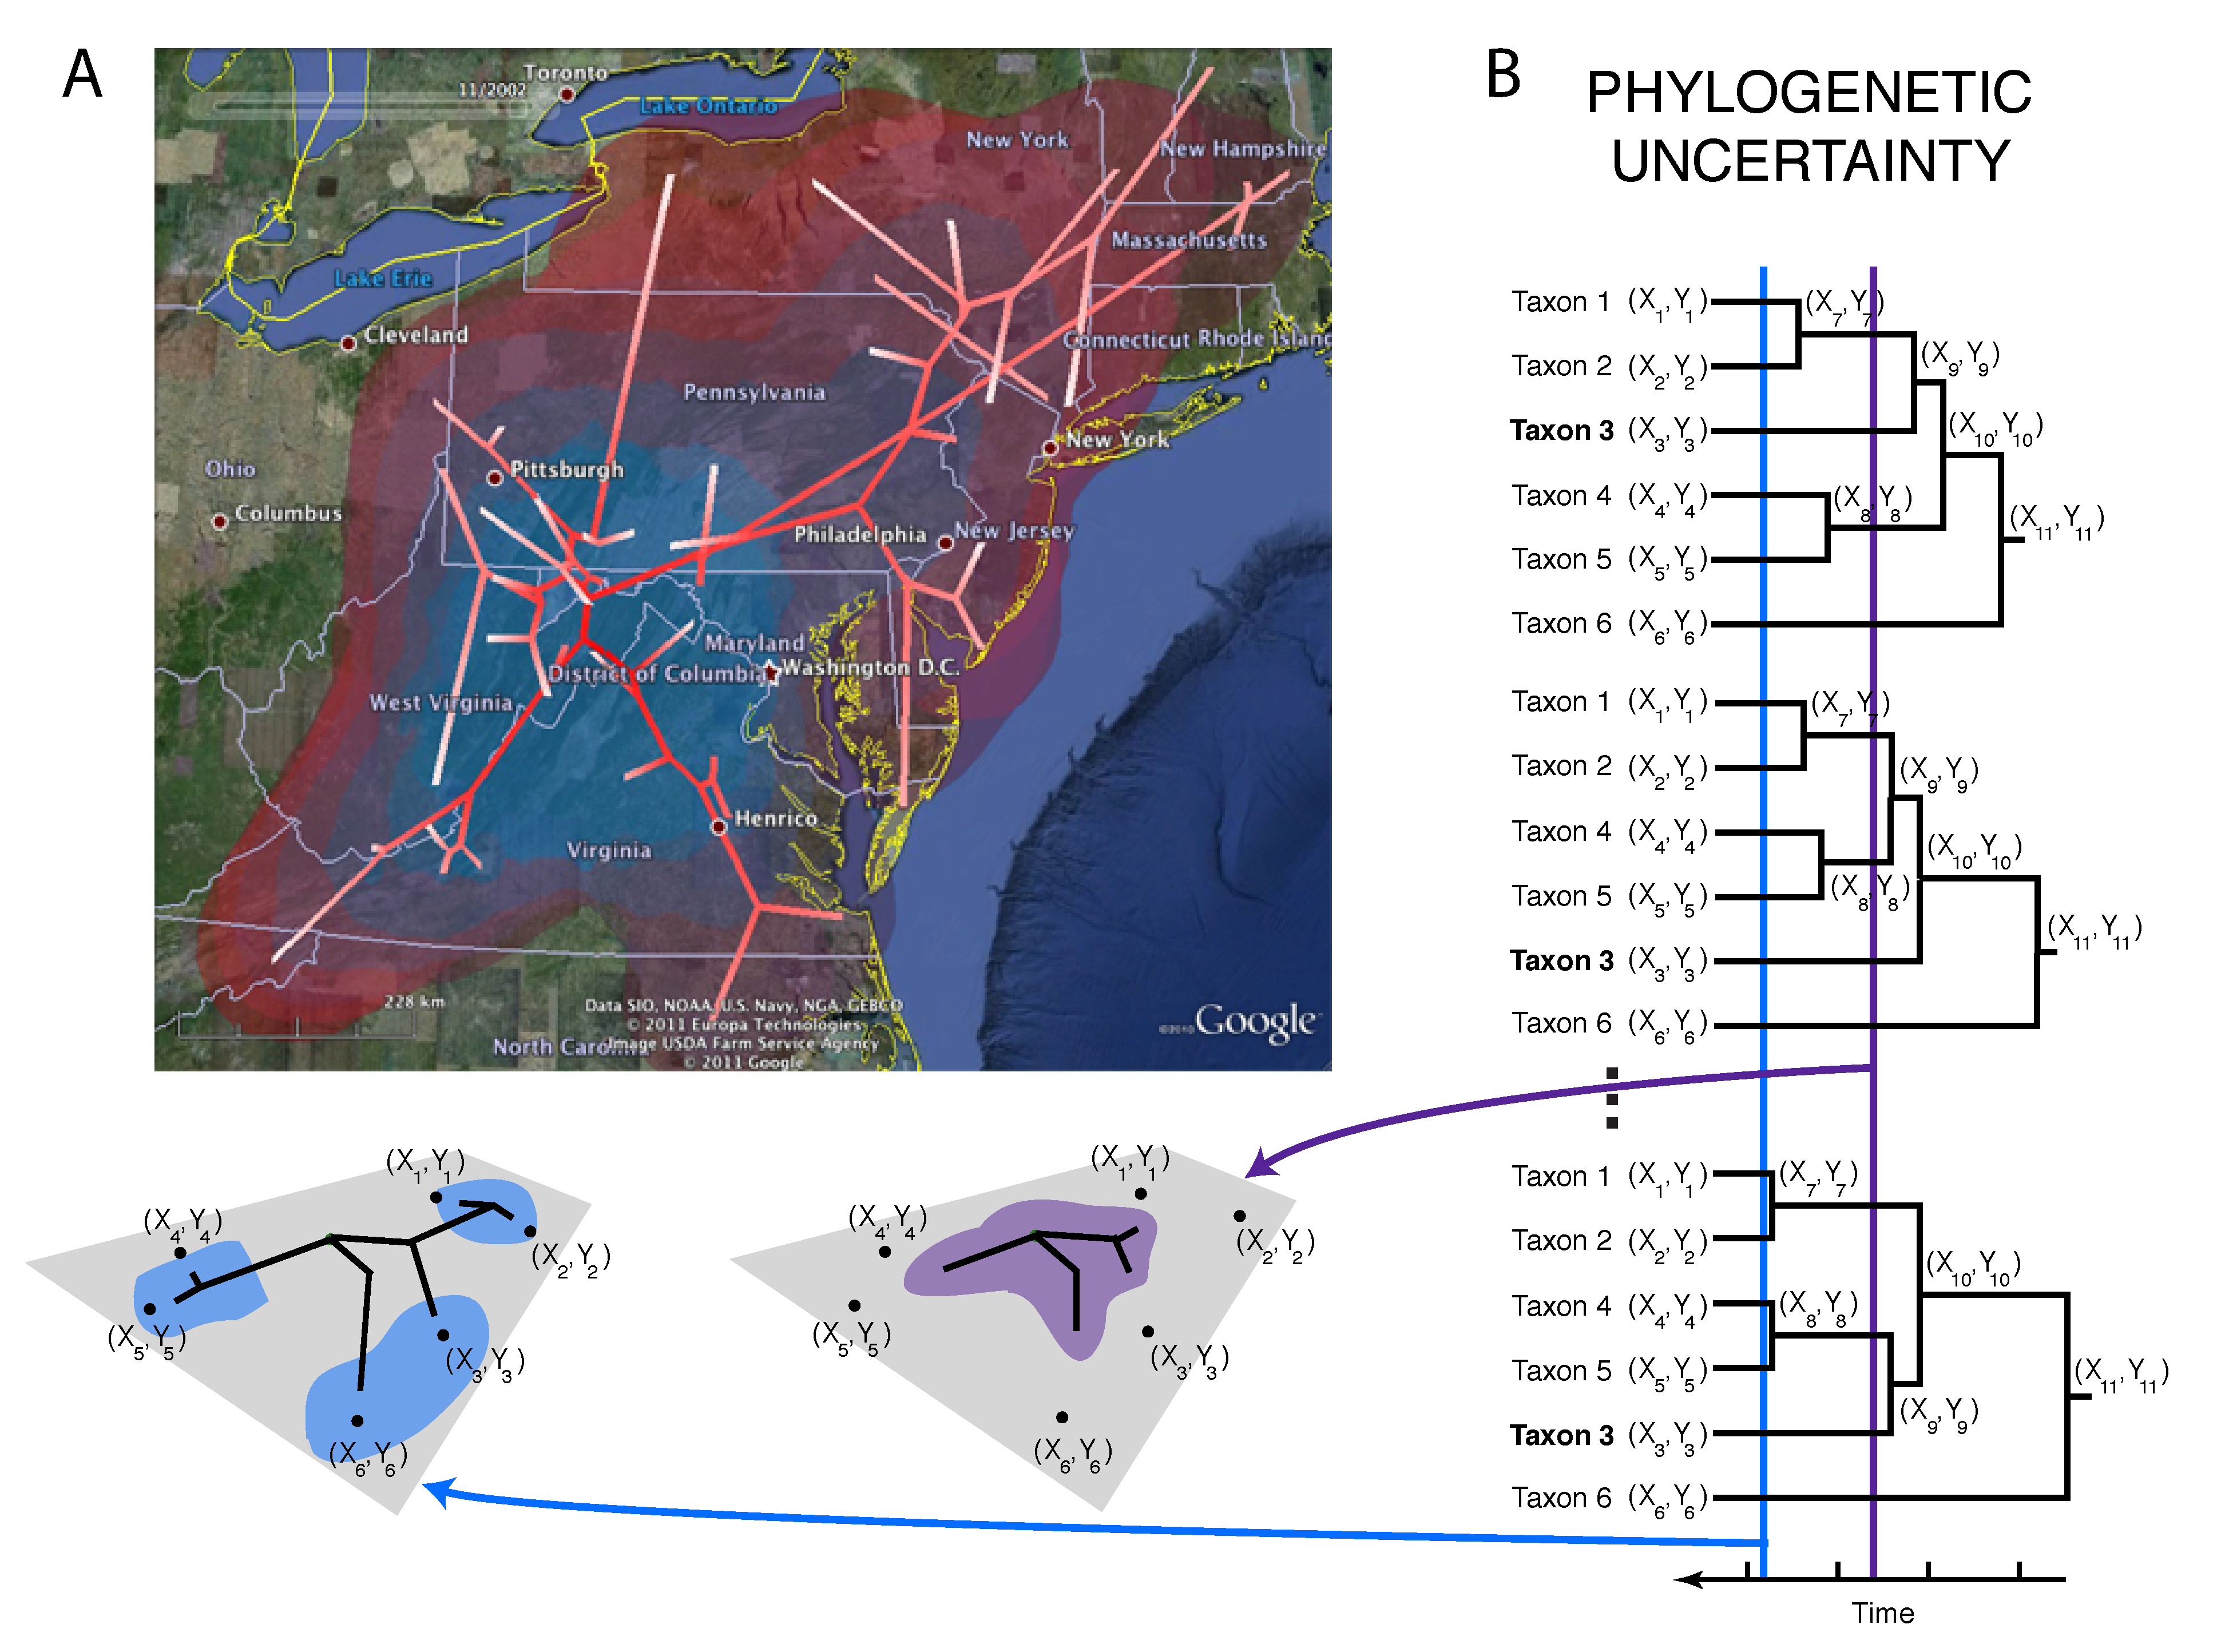
\includegraphics[scale=0.2]{continuous.pdf}
\caption{
{ \footnotesize 
{\bf Visualizing continuous phylogeographic reconstructions with uncertainty.} 
A. Example visualization in Google Earth based in estimates obtained from a real data set. B. Conceptual representation of visualizing uncertainty by time slicing a posterior distribution.
} % END: footnotesize
}
\label{fig:cont}
\end{figure}

%Two time slices are shown as an example for the continuous diffusion through time. 
%An example tree is mapped in continuous space, based on average bivariate coordinates for the internal nodes. 
%The uncertainty at any time-slice is depicted using credible contours, obtained from slicing the complete posterior distribution of location-annotated trees, sampled by BEAST.
%SPREAD supports also 2D alternatives of such projections.

\paragraph{}
In the discrete mapping, where each state represents a point location, similarly easily interpretable projections including uncertainty are harder to obtain.
Only branches that accommodate a state transition, according to the modal estimates at the parent and descendent node, can be distinguished and are projected as arcs, as depicted in Figure~\ref{fig:discrete}.
This illustrates a restrictive assumption of discrete phylogeographic inference, i.e. that all nodes are assumed to have lived in the locations from which samples were obtained.
Branches that maintain a particular state according to the parent and descendent node estimate can be displayed by a circle with a diameter proportional to the number of branches maintaining that state at any point in time.
The uncertainty associated with the node estimates in different posterior trees is however difficult to represent.
%The circle diameter reflects the number of branches that maintain a single state according to the parent and descendent node state.

\begin{figure}[h!]
\centering
\includegraphics[scale=0.4]{discrete}
\caption{
{ \footnotesize 
{\bf Phylogeographic visualization of viral spread in discrete space.} 
A. Conceptual representation of time-slicing a phylogeny and projecting the part of the tree up to time $t_{1}$ and $t_{2}$ respectively. 
B. An example projection of influenza H5N1 over time in Google Earth for two different segment phylogenies. % (hemagglutinin and neuraminidase in green and magenta respectively).
} % END: footnotesize
}
\label{fig:discrete}
\end{figure}

% now highlight some of the future perspectives
\subsection{Future perspectives}

With over a hundred citations by the time of writing this thesis, the original manuscript presenting SPREAD (\citet{Bielejec2011}, see Chapter \ref{chap:spread}) indicates a clear need for a package that can visualize phylogeographic diffusion processes inferred using Bayesian methods.
With that responsibility in mind we will continue to support SPREAD by adding new functionalities and making more analyses available to the practitioner.
The next major release of the software will be aimed at a thorough re-write of SPREAD's internal engine, which will hopefully result in a more stable and interactive package.
% Specifically we will target many of the feature requests, for example the ability to instantenously alter line and polygon coloring without the need to re-compute the analysis.

% outputting KML and web interfaces
\paragraph{}
The ability to output time-stamped KML documents which can then be played as animations is one of the most important functionalities of SPREAD and a major source of its popularity.
Future releases will continue to support that function, yet we will also add the ability to produce animated documents which can be embedded in webpages, viewed on mobile devices or locally on web browsers.
In our digital age, web visualization ensures accessibility and avoids the need to design proprietary software and plug-ins. We propose to merge data visualization concepts, interactive design and web development using D3 (\url{d3js.org}), a powerful JavaScript library for custom, web-based visualization. 
We will aim for a general visualization tool that maps the evolutionary patterns of traits with their uncertainty over time in their appropriate space. 
% For preliminary examples of interactive visualization see \url{http://justsz.github.io/pandemix/h9n2_AR.html}


%PL: you could also mention compatibility with BEAST2 and take this as an opportunity to describe the current situation of divergence in the two beast versions and parallel development for both.. the reader might be interested in this.
\paragraph{}
\cite{Pybus2012} recently introduced a conceptual link between phylogeography and spatial ecology, demonstrating that large-scale invasion dynamics, traditionally estimated using time-consuming field ecology methods, can be quantified from increasingly inexpensive molecular data.
We plan to make these new analyses available as part of SPREAD, with the possibility to produce spatial statistics (dispersal rate, wavefront, diffusivity), which can be extracted from the posterior distribution of BEAST trees by slicing each phylogeny at multiple times and summarizing the resulting distributions.
The new release of SPREAD will also have a Command Line Interface in support of pipelining large repetitive analyses, producing scripts or calling SPREAD from interpretable languages like R \citep{RCran} or Python.


%%%%%%%%%%%%%%
%---PIBUSS---%
%%%%%%%%%%%%%%
\section{Areas of improvement for the {\bussname} simulator software\label{sec:buss_future}}

Except for empirical models of evolution, most phylogenetic methods build on mathematical theory that predicts outcomes conditional on a set of assumptions.
How well these models fit to real data, and how robust they are to the violations of these assumptions remains to a large extent an open question.
Furthermore, biological systems targeted by phylogenetic studies undergo complex processes, which may be difficult to distinguish from stochastic error in the data.
Rapidly evolving viruses, which are the main interest of the research presented in this thesis, are subject to mutation, natural selection and spatial diffusion.
For most of the molecular epidemiology data-sets, the true underlying evolutionary process that generated the observations remains unknown or particular aspects of the process remain difficult to test.
For all these reasons, the is a need to develop flexible simulation software that allows evaluating the performance of phylogenetic and phylogeographic estimators.

% adding more models
\subsection{Model availability}

Our phylogenetic simulation software, $\pi$BUSS, presented in Chapter \ref{chap:pibuss} allows to fabricate evolution under a variety of coalescent, nucleotide, amino-acid and codon substitution models, as well as diffusion models, combined with various molecular clock specifications.
In addition it offers the ability to specify different models for arbitrary partitioning schemes.
We are committed to extend the collection of available models and data types even further in future releases of $\pi$BUSS.
We aim at matching the model richness available for inference in BEAST, and supplying every model available for inference with its simulation counterpart.
Specifically, we will implement simulation counterparts for the flexible coalescent priors, like the skyline \citep{Drummond2005} or skyride \citep{Minin2008b} models.
We are also considering various extensions of biologically realistic codon models with across-site and across-branch variation for future releases of the software.
Currently, simulation of trait data in $\pi$BUSS is limited to discrete univariate traits.
With a growing interest in multivariate trait data, not only in molecular epidemiology but in comparative biology in general, there will arise a need to simulate under continuous diffusion models.
We plan to implement several models to this effect, such as Brownian diffusion models, relaxed random walk models and further extensions that model drift dynamics.

\subsection{Graphical user interface and BEAUti integration}

% gui for more complex models
We will continue to support model specification via a 
%The models' specification will continue to be available via the
user-friendly Graphical User Interface (GUI), which allows to setup a simulation by choosing models from drop-down menus, partitioning data in tables and parsing parameters from text fields in an intuitive fashion.
Time-heterogeneous models, for which evolutionary parameters change both across different lineages (see Subsection~\ref{sub:dpp}) as well as models of pan-lineage change (see Chapter \ref{chap:epoch}) will be supported by dedicated panels, therefore avoiding the need to manually edit XML files.
% beauti integration
In addition to the Command Line Interface for scripting purposes, $\pi$BUSS is in a sense similar to the BEAUti software tool, which assists BEAST users in setting up their analysis through a user-friendly GUI.
We will proceed along that path and provide even closer integration between the two programs in order to facilitate the generation of joint simulation-analysis XML documents in which fabricated data is instantly passed on to the BEAST XML parsers for inference.

% indel models
\subsection{Simulation of insertion deletion events}
%The extent of this impact will depends on the position of the event in the coding regions of the genome.
% FB: check if I'm not talking out of my ass here:
% PL: you are :), an indel that disrupts the reading frame makes the protein dysfunctional. If not, it still has a high probability of affecting the protein function
%When an integer multiple of a codon triplet is inserted or deleted it means that one or more amino acids are inserted or deleted leaving the protein function unchanged.
%In the case of one or two indel events the resulting gene usually codes for a different protein with different amino-acids.

In molecular evolution, not only substitution processes (Subsection \ref{sub:subst_models}), but also insertions and deletions (indels) provide a mechanism for generating genetic diversity.
Indel mutations are well known to have a significant impact on molecular evolutionary processes \citep{Fletcher2009}, and small viral genomes may be particularly sensitive to them.
Indels are not only of interest because of their evolutionary consequences, but they are also important to accurately position by alignment procedures.
Realistic indel simulation requires however specific stochastic models.
Standard modeling assumptions, such as those used in CTMC substitution models (see Subsection~\ref{sub:subst_models}), are not realistic for indel events. %PL:  point out which ones. Reversibility seems a major one
Future releases of $\pi$BUSS will aim at implementation stochastic processes for indel evolution.
%PL: I deleted the stochastic doll model as it doesn't seem to be the first to think about. It is a specific acquisition-loss process that allows acquiring a trait once and then independently loosing that trait on multiple occasions (but never acquiring it anymore). A bit more on models specifically dealing with indel evolution and some references would suit better here. Quickly scan some papers to drop something on them -- you may get questions on this anyway.

Just like substitutions, indels are discrete event occuring in a real time.
By convention, following \cite{Thorne1991} the insertion-deletion events are typically presented as links separating character sequence bases (see Figure~\ref{fig:indels}).
Indels are characterized by two parameters.
The length represents the number of blocks inserted or deleted, where each block is an integer multiple of 1 for nucleotide or an integer multiple of 3 for codons space. 
Conversely the location is the position in the sequence where the blocks of characters are inserted or the position where the deletion begins.

\begin{figure}
\centering
$$\bullet\; C\;\star C\;\star\; A\;\star\; C\;\star\; T\;\star$$
\caption{
{ \footnotesize 
{\bf DNA sequence CCACT of length $L=5$, with $L+1$ links that separate the characters.} 
By convention to the right of each base there is a \textit{normal link} ($\star$); the leftmost base has an \textit{immortal link} to itself ($\bullet$), ensuring that an insertion can occur at position $l=0$.
} % END: footnotesize
}
\label{fig:indels}
\end{figure}

\cite{dawg} models indel sizes \textit{i.a.} using a negative binomial distribution and a power law, truncated at some user specified, maximum indel size $M$.
\cite{Benner1993} notes that the power law (the Zipfian distribution, \cite{Gonnet1991}) follows the empirical gap lengths distribution. 

If by $\lambda_{I}$ we denote the insertion rate at a location, then the waiting times until an insertion occurs are exponentially distributed with rate $\lambda_{I}(L+1)$.
Insertions are then drawn from the stationary distribution $\mathbf{\Pi}=\{\pi_{i},\ i\in\mathcal{E}\}$ of the underlying substitution model.

The procedure of \cite{dawg} simulates deletion by assuming that the simulated sequence, of length $L$ lies within a larger sequence of length $N$, where $L\ll N$.
The maximum allowed deletion spans for $M$ blocks, such that $M \ll N$.
This ensures that the deletions can happen at the end of the sequence.
A deletion of an arbitrary size $u$ happening in the larger sequence will result in deletions in the subsequence, if it begins at one of the L sites of the smaller sequence, or one of the $u-1$ sites preceding the subsequence.
Deletions are assumed to appear uniformly along the larger sequence, therefore the probability of a deletion of size $u$ in the larger sequence deleting some part of the smaller sequence is $\frac{u-1+L}{N}$.
If $\lambda_{D}$ is the rate of deletion per location then the waiting time for a deletion in a smaller sequence is exponentially distributed with rate $\lambda_{D}(u-1+L)$ \citep{dawg}.



%%%%%%%%%%%
%---HPC---%
%%%%%%%%%%%
\section{High performance computing\label{sec:hpc}}

The ever growing availability of molecular data produced by high-throughput sequencing brings about formidable challenges for analyses, and it is even dubbed the biggest challenge for the field of virology and molecular epidemiology. 
High performance computing (HPC) will become even more critical to address this challenge.
%High performance computing (HPC) tasks are characterized as needing large amounts of computing power, and teh field is interested in reducing the time to complete an individual job.
Here, we discuss several architectures that are used for high performance statistical phylogenetics. 

\subsection{Parallel computations}

John von Neumann in his famous `First Draft of a Report on the EDVAC' \citep{vonNeumann1945} describes a sequential program, the execution of which can be followed by sequentially stepping through the code.
%
%\begin{remark}{The First Draft of a Report on the EDVAC}
%The First Draft of a Report on the EDVAC, or simply First Draft for short, is an incomplete, $101$-page document which was written by John von Neumann during his daily commutes by train.
%% \begin{center}
%% First Draft of a Report on the EDVAC
%% by John von Neumann, 
%% Contract No. W-670-ORD-4926, 
%% Between the United States Army Ordinance Department 
%% and the University of Pennsylvania Moore School of Electrical Engineering 
%% University of Pennsylvania 
%% June 30, 1945
%% \par\end{center}
%\begin{figure}[H]
%\centering
%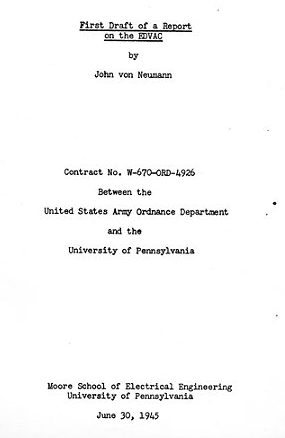
\includegraphics[scale=0.5]{first_draft}
%\caption{
%{ \footnotesize 
%{\bf The title page of the report.}
%} % END: footnotesize
%}
%\label{fig:vonNeumann}
%\end{figure}
%
At that time von Neumann was working as a consultant for the U.S. Army's Ballistics Research Laboratory, which played an important role in the early history of computers, developing and building several generations of first computers.
The report itself provided the first description of a computer in the modern sense, capable of running progams stored in its memory, hence the name \textit{Electronic Discrete Variable Automatic Computer}.
%Later it was a cause of many controversies, as the lead developers of ENIAC (predecessor of EDVAC) and EDVAC, John Mauchly and John Presper Eckert were not listed as authors, leading to all the credit being attributed to von Neumann.
%\end{remark}

Traditionally a vast majority of programs were written as sequential code, following von Neumanns design, which proved to be working well for the scientific community for many years.
This relates to an observation, which later came to be known as Moore's law, predicting the trend in chip performance as doubling roughly every $18$ months.
%As captured by an observation that later came to be known as Moore's law, chip performance was predicted to double roughly every $18$ months.
Figure~\ref{fig:moore} shows how, during the time of $15$ years, the hardware performance and improvements in compiler technology provided a speedup by a factor of $80$.
For practical purposes this meant that just by updating the hardware architecture and compilers increasingly bigger problems could be tackled, without ever changing the code-base of the numerical programs. 
The same software would simply run faster with the introduction of new generations of processors and new versions of compilers.
%This has created a positive cycle for the computer industry.
However, during the last two years in the plot this gain is no longer visible\footnote{The free lunch is over!}.
Due to hardware limitations, and problems with heat dissipation, we are now at the limit of how many transistors can be put into integrated circuits, which determines CPU performance.
As a consequence, serial computations on new CPUs no longer benefit from the same increases in speed and performance.

\begin{figure}[h!]
\centering
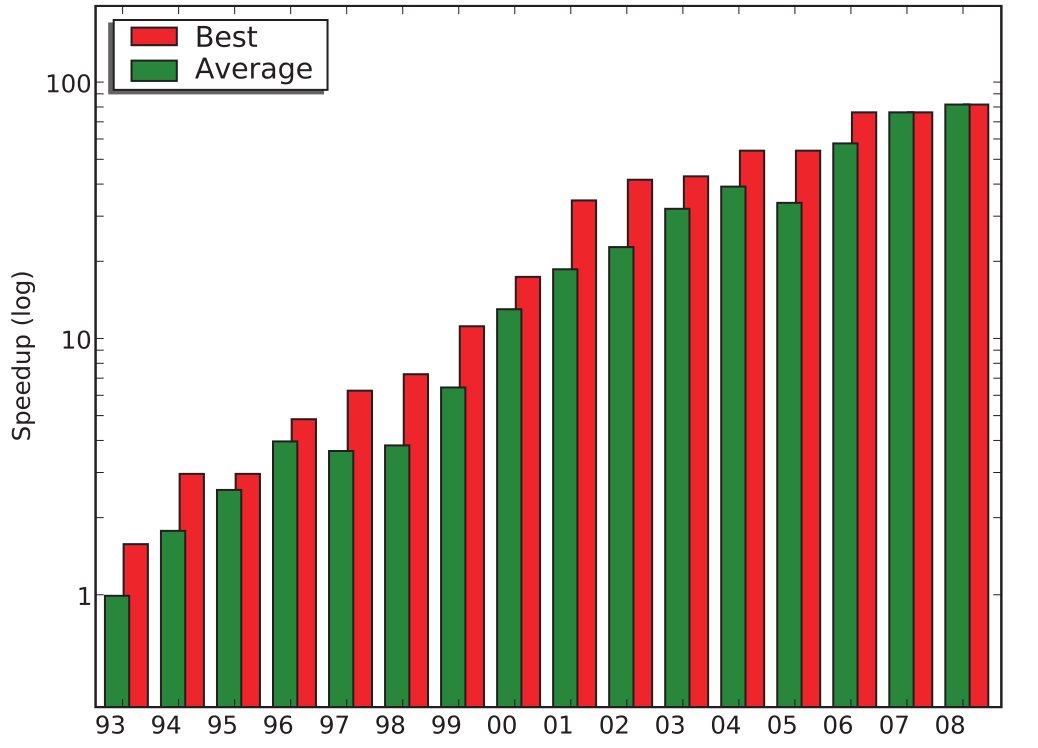
\includegraphics[scale=0.2]{moore}
\caption{
{ \footnotesize 
{\bf Performance gains of a numerical code benchmarked on a single CPU core over the course of 15 years (PDE solver FeatFlow, \citep{Turek1999}).}
Last two years have seen only a marginal speed-up, and correspond to the shift to multicore architectures.
} % END: footnotesize
}
\label{fig:moore}
\end{figure}


\paragraph{}
Fortunately the increasing availability of parallel processing hardware offers a solution for almost all data intensive computations.
This implies that software applications will continue to benefit from performance improvements as long as they target the new generation of parallel microprocessors in which multiple threads cooperate to jointly complete the work faster.
Computers employing parallel architectures are becoming more widespread, and can take a form of supercomputer clusters, but also inexpensive desktop multiprocessors or workstations equipped with parallel accelerators that can be geared specifically towards scientific computing.
This brings about an increasing need for parallelizing programming code, something referred to as the \textit{concurrency revolution} \citep{Sutter2005}.

% two roads: many core and multi core
\subsection{Many-core versus multi-core}

%Emerging areas of research, such as computational biology have all implications for algorithms and software development.
To capitalize on the vast amounts of data that are now available, future development of phylogenetic software should target high performance parallel computing devices.
To properly leverage this computation power, the burden of improving the performance is, at least partially, shifted from hardware vendors to software developers.
Writing and optimizing massively parallel code requires a thorough understanding of the underlying architecture, associated libraries and APIs and the correct use of the performance assessment tools.

\paragraph{}
Currently it seems that the semiconductor industry has established two, \textit{nomen set omen}, parallel paths for designing multiprocessors.
The \textit{multicore} path began with the idea of putting two CPU cores on the same chip.
This approach means that the current clock speed of a single core remains the same, but at the same time the vendors are approximately doubling the number of effective cores with every new generation.
In contrast, the \textit{many-core} path focuses on increasing the throughput of parallel applications by using large numbers of much smaller and simpler cores, and again approximately doubling the number of cores that is put on every new generation of devices. 
NVIDIA's GPUs are an exemplar of such many-core devices.
GPUs \citep{Nickolls2008} are making a big impact on the scientific computing, which falls under the term of general-purpose computing on graphics processing units (GPGPU).
%Because modern GPU devices are designed to maximize throughput of a given computation they are capable of achieving impressive peak performances (see Subsection~\ref{sub:fine_grain}).
The most important factor that contributed to the wide adoption of GPUs for scientific computing is the fact that substantial performance improvements are relatively easily affordable. 
Furthermore the parallel computing architecture comes with a variety of libraries, tools and extended C language to leverage the GPGPU capabilities, including NVIDIA's CUDA framework and various implementations of the OpenCL (Open Computing Language) standard.

% beagle
\paragraph{}
%\cite{Suchard2009} have pioneered the use of GPGPU for statistical phylogenetics.
By developing the BEAGLE high-performance library for  evaluating phylogenetic likelihoods of molecular sequence evolution, \cite{Suchard2009} 
have pioneered the use of GPGPU in statistical phylogenetics.
%This work has resulted in the development of the Beagle high-performance library for  evaluating phylogenetic likelihoods of biomolecular sequence evolution \citep{Ayres2012}.
BEAGLE can make use of other highly-parallel processors beside GPUs and is also capable of calling SSE (Streaming SIMD Extensions) as well as AVX (Advanced Vector Extensions) vector instructions, thus achieving improved performance on the current generation of Intel microprocessor architectures.
The BEAGLEAPI \citep{Ayres2012} can currently be used by a range of phylogenetic software tools, such as MrBayes (\url{http://mrbayes.sourceforge.net}), Garli (\url{https://garli.googlecode.com}), PhyML (\url{https://phyml.googlecode.com}) and BEAST.

\paragraph{}
The use of Graphics Processing Units for scientific computing does not come without some caveats.
Recent NVIDIA GPU chips intended for the high-margin PC gaming market, the GeForce 600 and 700 series, have had their double-precision capabilities crippled.
This means that the scientific community interested in high-precision computations would have to turn towards more expensive Quadro and Tesla cards, or the GeForce GTX Titan card, instead of cost-sensitive consumer-class devices.

\paragraph{}
Perhaps more important is the fact that the host-device scheme, in which the GPUs operate, represents a bottleneck that hampers the effective usage of GPU devices.
In a typical workflow of a GPGPU program both the host and device memory need to be allocated, host memory needs to be copied to the device, and after executing a GPU kernel the results need to be copied back to the CPU memory.
The copying happens over a PCI Express bus, a point-to-point serial interface organized in the form of bi-directional lanes (each lane transmits the data in one direction).
The typical bandwidth of a modern card ranges around $300$ GB/c, while a PCI express bus v3.0 has a theoretical peak speed of 15.75 GB/s in each direction.
This bottleneck can severely affect the potential for speed increases on GPUs, in fact the impressive peak-performances reported by the vendors are almost never achieved in real-world applications.

% karma/ maxwell 
\subsection{Emerging architectures}

% Perhaps the emerging Heterogeneous System Architecture (HSA) will offer and interesting solution to this problem.
While current CPUs and GPUs are designed as separate devices, requiring an application to explicitly copy data from CPU to GPU and then back again, a Heterogeneous System Architecture (HSA) is geared towards having a single, unified memory address space for all the data structures.
This means that multiple compute tasks can work on the same memory regions avoiding the bottlenecks mentioned above.
As an example, NVIDIAs Tesla accelerator cards based on the Maxwell architecture aim at an integrated ARM CPU. %of its own\footnote{Barcelona Supercomputing Center in Spain has been working on a prototype ARM-GPU supercomputer for a few years now.}.
ARM is a family of processors based on the RISC (Reduced Instruction Set Computing) architecture, best known from portable, battery-powered devices such as smartphones or tablets. 
Other vendors are also working on similar hybrid solutions.

\paragraph{}
Another interesting avenue, and perhaps a competitor to the already presented architectures geared to scientific computing, are the field-programmable gate arrays (FPGA, \citet{Kuon2008}).
Although not a new design, recent developments and renewed interest in these chips justify discussing them here.
FPGAs are chips that can be configured at low cost by the end-customer after being manufactured, hence the name.
FPGAs are build from logic blocks, memory elements and a set of interconnects, which can be programmed and reconfigured to perform arbitrarily complex logical operations.
% This means that they can be reconfigured at low  cost to best suit the problem that is at hand.
Typical modern FPGAs employ bi-directional data lanes, with very fast I/O (Input/output), and in addition, many FPGAs can be re-programmed during run-time. 
%
%\begin{remark}{Road To Riches}
%% https://www.reddit.com/r/Bitcoin/comments/18q2jx/eli5_bitcoin_mining_xpost_in_eli5/
%FPGAs are a very fast and power efficient way to implement the SHA256 hashing algorithm, or mining Bitcoins in simple words.
%Various companies are offering configured FPGA chips specific to the task, there also exists an Open-Source implementation of software for various FPGA systems.
%\end{remark}
%
The reconfiguration at low cost allows targeting a specific problem at hand.
%Therefore their main advantage comes from the fact that they can be reconfigured at low  cost to best suit a specific problem at hand.
The first attempts at extending the BEAGLE library to FPGA architecture have recently emerged \citep{Jin2013}.

\paragraph{}
In the light of these advances it is fair to say that we are entering a new era of parallel computing.
The barrier for writing parallel code lowers with every generation of parallel devices.
Researchers all over the world are starting to develop new models and algorithms that can benefit from this revolution.
Hardware vendors are designing new devices that improve power efficiency, bandwidth and clock speed with every new generation.
All these improvements come at the right moment.
The advent of next generation sequencing data has lead to the generation of complete genome sequences in short time and at relatively low costs.
Nowadays, it is not uncommon to work with datasets including whole genomes of organisms.

Complex, biologically-realistic models that target this information also bring about new computational challenges.
Models with large state spaces, such as codon models discussed in Subsection~\ref{sub:dpp} are an example of such a challenge.
More research will be needed to mitigate the imminent computational burdens that come with novel modeling approaches and high-throughput sequencing. 
This will open up new opportunities to analyze data in almost real time, and by coupling molecular sequence data with geographical information, to trace the spread of emerging epidemics and instantly identify potential outbreak locations as well as the drivers of viral spread.  
Although it is hard to make any specific predictions, it will be very interesting to see where the future will lead to at the cross-section of data-plenty and high-performance computing and how this will advance infectious disease research.
















